\chapter{The RFSM language}
\label{cha:language}

This section describes the syntax and semantics of the \emph{standard} RFSM language in a more
systematic, but informal, way. The corresponding formalized descriptions are given in the reference
manual.

\section{Programs}
\label{sec:programs}

A RSFM program is made of successive sections, containing, respectively 
\begin{itemize}
\item type declarations,
\item constant declarations,
\item function declarations,
\item FSM model definitions,
\item global object definitions,
\item FSM instanciations.
\end{itemize}

Each section is optional\footnote{Though, obviously, a program with no model definition, and hence
  no FSM instanciation, is of little interest.} but their must appear in the order given above.

\section{FSM models}
\label{sec:fsm-models}

% The general form of an FSM model is given in listing.~\ref{lst:fsm-model-gen}.
% \begin{lstlisting}[language=Rfsm,frame=single,caption=Overall syntax for FSM models,label=lst:fsm-model-gen]
% fsm model <@\emph{parameter declarations}@> @\emph{name}@ (
%      @\emph{io declaration}@
%   {
%   states: @\emph{state declaration}@;
%   vars: @\emph{variable declaration}@;
%   trans: @\emph{transition descriptions}@;
%   itrans: @\emph{initial transition description}@;
%   }
% \end{lstlisting}
% where
% \begin{itemize}
% \item \emph{name} is the name of the defined model,
% \item \emph{parameter declarations} is an optional list of generic parameters,
% \item \emph{io declarations} list the inputs and outputs of the FSM,
% \item \emph{state declarations} list the states of the FSM,
% \item \emph{variable declarations} is an optional list of internal variables,
% \item \emph{transition descriptions} describe all the transitions of the FSM,
% \item \emph{initial transition description} describes the initial transition of the FSM.
% \end{itemize}

An FSM model, introduced by the \verb|fsm model| keywords, describes the interface and behavior of a
\emph{reactive finite state machine}. A reactive finite state machine is a finite state machine
whose transitions can only be caused by the occurrence of \emph{events}.

\begin{center}
\framebox{\lstinline[language=Rfsm]|fsm model <interface> { <body> }|}
\end{center}

\medskip The \textbf{interface} of the model gives its name, a list of parameters (which can be
empty) and a list of inputs and outputs. All parameters and IOs are typed (see
Sec.~\ref{sec:types}). Inputs and outputs are explicitely tagged. An IO tagged \verb|inout| acts
both as input and output (it can be read and written by the model). Inputs and outputs are listed
between \verb|(...)|. Parameters, if present are given between \verb|<...>| and allow the
definition of \emph{generic} models. Examples :

\begin{center}
\example{\lstinline[language=Rfsm]|fsm model cntmod8 (in h: event, out s: int<0..7>) \{ ... \}|}
\end{center}

\begin{center}
\example{\lstinline[language=Rfsm]|fsm model gensig<n:int> (in h: event, in  e: bit, out s: bit) \{ ... \}|}
\end{center}

\begin{center}
\example{\lstinline[language=Rfsm]|fsm model update (in top: event, inout  lock: bool) \{ ... \}|}
\end{center}

\medskip
The model \textbf{body}, written between \verb|{...}|, generally comprises four sections :
\begin{itemize}
\item a section giving the list of \emph{states},
\item a section introducing local (internal) \emph{variables},
\item a section giving the list of \emph{transition},
\item a section specifying the \emph{initial transition}.
\end{itemize}

Each section starts with the corresponding keyword (\verb|states:|, \verb|vars:|, \verb|trans:| and
\verb|itrans:| resp.) and ends with a semi-colon.

\begin{center}
\framebox{\lstinline[language=Rfsm]| fsm model ... ( ... ) \{ states: ...; vars: ...; trans: ...; itrans: ...; \}|}
\end{center}

\subsection{States}
\label{sec:states}

The \verb|states:| section gives the set of internal states, as a comma-separated list of
identifiers (each starting with a uppercase letter). Example :

\begin{center}
\example{\lstinline[language=Rfsm]|states: Idle, Wait1, Wait2, Done;|}
\end{center}

Values for outputs can be attached to states using the \verb|where| keyword. When several
assignements are attached to the same state, they are separated using the \verb|and| keyword.

\begin{center}
\example{\lstinline[language=Rfsm]|states: Idle, Wait1 where s1=0, Wait2 where s1=1 and s2=0, Done;|}
\end{center}

\subsection{Variables}
\label{sec:variables}

The \verb|vars:| section gives the set of internal variables, each with its type. Example :

\begin{center}
\example{\lstinline[language=Rfsm]|vars: cnt: int, stop: bool;|}
\end{center}

The type of a variable may depend on parameters listed in the model interface. Example

\begin{center}
\example{\lstinline[language=Rfsm]|fsm gensig<n: int> (...) \{ ... vars: k: int<0:n>; ... \}|}
\end{center}

The \verb|vars:| section may be omitted.

\subsection{Transitions}
\label{sec:transitions}

The \verb|trans:| section gives the set of transitions between states. Each transition is denoted

\begin{center}
\framebox{\lstinline[language=Rfsm]{| src_state -> dst_state on ev when guards with actions}}
\end{center}

where
\begin{itemize}
\item \emph{src\_state} and \emph{dst\_state} respectively designates the source state and destination state,
\item \emph{ev} is the event trigerring the transition,
\item \emph{guards} is a set a enabling conditions,
\item \emph{actions} is a set of actions performed when then transition is enabled.
\end{itemize}

\medskip The semantics is that the transition is enabled whenever the FSM is in the source state,
the triggering event occurs and all conditions evaluate to true. The associated actions are then
performed and the FSM moves to the destination state.

\medskip
The triggering event must be listed in the inputs.

\medskip
Each condition listed in \emph{guards} must evaluate to a boolean value. The guard is true if
\emph{all} conditions evaluate to true (conjonctive semantics).
The guards may involve inputs and/or internal variables.

\medskip
The guard can be empty. In this case, the transition is denoted
\begin{center}
\framebox{\lstinline[language=Rfsm]{| src_state -> dst_state on ev with actions}}
\end{center}

\medskip The \textbf{actions} associated to a transition consists in modifications of the outputs
and/or internal variables or emissions of events. Modifications of outputs and internal variables
are denoted

\begin{center}
\framebox{\lstinline[language=Rfsm]{id := expr}}
\end{center}

where \emph{id} is the name of the output (resp. variable) and \emph{expr} an expression involving
inputs, outputs and variables and operations allowed on the corresponding types.

\medskip
The action of emitting of an event  is simply denoted by the name of this event.

\medskip
Examples :

\begin{center}
\example{\lstinline[language=Rfsm]'S0 -> S1 on top '}
\end{center}

In the above example, the enclosing FSM switches from state \verb|S0| to state \verb|S1| when the
event \verb|top| occurs. 

\begin{center}
\example{\lstinline[language=Rfsm]'Idle -> Wait on Clic with ctr:=0, received'}
\end{center}

In the above example, the enclosing FSM switches from state \verb|Idle| to state \verb|Wait|, resetting the internal variable
  \verb|ctr| to 0 and emitting the event \verb|received| whenever an event occurs on its \verb|Clic| input.

\begin{center}
\example{\lstinline[language=Rfsm]'Wait -> Wait on Top when ctr<8 with ctr:=ctr+1'}
\end{center}

In the above example, the enclosing FSM stays in state \verb|Wait| but increments the internal
variable \verb|ctr| whenever an event \verb|Top| occurs and that, \emph{at this instant}, the
value of variable \verb|ctr| is smaller than 8. 

\medskip
Expressions may also involve the C-like ternary conditional operator \verb|?:|.
For example, in the example below, the enclosing FSM stays in state \verb|S0| but updates the variable \verb|k|
at each occurrence of event \verb|H| so that is incremented if its current value is less than 8 or
reset to 0 otherwise.

\begin{center}
\example{\lstinline[language=Rfsm]'S0 -> S0 on H with k:=k<8?k+1:0'}
\end{center}

\medskip
The set of actions may be empty. In this case, the transition is denoted :

\begin{center}
\framebox{\lstinline[language=Rfsm]{src_state -> dst_state on ev when guard}}
\end{center}

\subsubsection*{Semantic issues}
\label{sec:semantic-issues}

\textbf{Sequential vs. synchronous actions}.
By default, actions are performed  \emph{sequentially}, i.e. one after the other. 
For example, if \verb|x| and \verb|y| are internal variables of the enclosing FSM and respectively
have values 1 and 0, then taking this transition

\begin{center}
\example{\lstinline[language=Rfsm]'S0 -> S1 on H with x:=x+1, y:=x*2'}
\end{center}

will assign them values 2 and 4 respectively, because the action \verb|x:=x+1| is performed before
the action \verb|y:=x*2|. 

This interpretation is the most intuitive one and naturally fits with software-based
implementations.
% There's actually another interpretation in which actions are not performed sequentially but
% \emph{synchronously}. In this case, all the expressions appearing on the right-hand-side of
% assignations are fisrt evaluated \emph{in parallel} and then, and only then, all the assignations
% are performed. Because the values of the variables occuring in the RHS expressions are those 
% \emph{before} the transition, the order in which the actions are performed does not matter in this
% case. In the example above, the values assigned to \texttt{x} and \texttt{y} will be 2 and 2
%   respectively. This interpretation more naturally fits to \emph{hardware-based} implementations,
% in which variables are implemented as \emph{signals} all updated synchronously at each clock cycle. 
% Switching to a synchronous interpretation is possible by invoking the \texttt{rfsmc} compiler with the
% \verb|-synchronous_actions| option. \textbf{Caveat}. This option is
% available when using the simulator and the VHDL backend but is
% currently not supported when using the C and SystemC backends.

\medskip
\textbf{Non-determinism and priorities}. 
The FSM models involved in programs should normally be \emph{deterministic}. In other words, a
situation where several transitions are enabled at the same instant should normally never arise. But
this condition may actually be difficult to enforce, especially for models reacting to several input
events. Consider for example, the model described in Listing~\ref{lst:rfsm-prio-pb}. This model
describes a (simplified) stopwatch. It starts counting seconds (materialized by event \verb|sec|)
as soon as event \verb|startstop| occurs and stops as soon as it occurs again.

\begin{lstlisting}[language=Rfsm,frame=single,numbers=left,caption=A program showing a potentially non-deterministic
  model,label={lst:rfsm-prio-pb},float]
fsm model chrono (
     in sec: event,
     in startstop: event,
    out aff: int)
  {
  states: Stopped, Running;
  vars: ctr: int;
  trans:
  | Stopped -> Running on startstop with ctr:=0; aff:=0
  | Running -> Running on sec with ctr:=ctr+1; aff:=ctr
  | Running -> Stopped on startstop;
  itrans:
  |-> Stopped;
  }

input StartStop: event = sporadic(25,70)
input H:event = periodic(10,10,110)
output Aff: int

fsm c = chrono(H,StartStop,Aff)
\end{lstlisting}

The problem is that if both events occur simultaneously  then
both the transitions at line 10 and 11 are enabled. In fact, here's the error message produced by
the compiler when trying to simulate the above program :

\small
\begin{verbatim}
Error when simulating FSM c: non deterministic transitions found at t=70:
	- Running -- H / ctr:=ctr+1; aff:=ctr -> Running
	- Running -- StartStop -> Stopped
\end{verbatim}
\normalsize

Of course, this could be avoided by modifying the stimuli attached to input \verb|StartStop| so that
the \texttt{StartStop} and \texttt{H} events are never emitted at the same time. But this is, in a
sense, cheating, since the \texttt{StartStop} event is supposed to modelize user interaction which
occur, by essence, at impredictible dates.

The above problem can be solved by assigning \emph{priorities} to transitions. In the current
implementation, this is achieved by tagging some transitions as ``high priority''
transitions\footnote{Future versions may evolve towards a more sophisticated mechanism allowing
  numeric priorities.}.  When several transitions are enabled, if one is tagged as ``high priority''
than it is automatically selected\footnote{If none (resp. several) is (resp. are) tagged, the
  conflict remains, of course.}. 

Syntaxically, tagging a transition is simply achieved by replacing the leading ``\verb+|+'' by a
``\verb|!|''.  In the
case of the example above, the modified program is given in
Listing~\ref{lst:rfsm-prio-solved}. Tagging the last transition is here equivalent to give to the
\verb|startstop| precedence against the \verb|h| event when the model is in state
\verb|Running|.

\begin{lstlisting}[language=Rfsm,frame=single,numbers=left,caption=A rewriting of the model defined
  in Listing~\ref{lst:rfsm-prio-pb}, label={lst:rfsm-prio-solved},float]
fsm model chrono (...)
  {
  ...
  trans:
    ...
    | Running -> Running on sec with ctr:=ctr+1; aff:=ctr
    ! Running -> Stopped on startstop  -- This transition takes priority on the others
  itrans: -> Stopped;
  }
...
\end{lstlisting}

\subsection{Initial transition}
\label{sec:initial-transition}

The \verb|itrans:| section specifies the initial transition of the FSM. This transition is denoted~:

\begin{center}
\framebox{\lstinline[language=Rfsm]{| -> init_state with actions}}
\end{center}

where \emph{init\_state} is the initial state and \emph{actions} a list of actions to be performed
when initializing the FSM. The latter can be empty. in this case the initial transition is simply
denoted~:

\begin{center}
\framebox{\lstinline[language=Rfsm]{| -> init_state}}
\end{center}

\subsection{Output values}

Output values can be set by either attaching them to states or by updating them on
transitions. For a given output \texttt{o}, attaching a value \texttt{v} to a state \texttt{S}, by writing

\begin{center}
\framebox{\lstinline[language=Rfsm]{states: S where o=v, ...}}
\end{center}

is equivalent to adding the action

\begin{center}
\framebox{\lstinline[language=Rfsm]{o:=v}}
\end{center}

to each transition ending at state \texttt{S}.

The compiler rejects models for which the value of an output is specified both with the former and
latter formulation. Stricly speaking, models for which the values specified by each formulation are
equivalent could be accepted, but this condition is statically undecidable in general (because
values assigned to outputs in transitions may depend of inputs).


\section{Inputs and outputs}
\label{sec:inputs-outputs}

Interface to the external world are represented by \verb|input| and \verb|output| objects.

\medskip
\step For outputs the declaration simply gives a name and a type~:

\begin{center}
\framebox{\lstinline[language=Rfsm]'output name : typ'}
\end{center}

\step For inputs, the declaration also specifies the \textbf{stimuli} which are attached to the
corresponding input for simulating the system.
\begin{center}
\framebox{\lstinline[language=Rfsm]'input name : typ = stimuli'}
\end{center}

There are three types of stimuli~:
periodic and
sporadic stimuli for inputs of type \verb|event| and value changes for scalar inputs.

\medskip
Periodic stimuli are specified with a period, a starting time and an ending time.

\begin{center}
\framebox{\lstinline[language=Rfsm]'periodic(period,t0,t1)'}
\end{center}

Sporadic stimuli
are simply a list of dates at which the corresponding input event occurs.

\begin{center}
\framebox{\lstinline[language=Rfsm]'sporadic(t1,...,tn)'}
\end{center}

Value changes are given as
list of pairs \verb|t:v|, where \verb|t| is a date and \verb|v| the value assigned to the
corresponding input at this date. 

\begin{center}
\framebox{\lstinline[language=Rfsm]'value_changes(t1:v1,...,tn:vn)'}
\end{center}

\medskip
Examples:

\begin{center}
\example{\lstinline[language=Rfsm]'input Clk: event = periodic(10,10,120)'}
\end{center}

The previous declaration declares \verb|Clk| as a global input producing periodic events with period 10, starting
  at t=10 and ending at t=100\footnote{Note that, at this level, there's no need for an absolute
    unit for time.}.

\begin{center}
\example{\lstinline[language=Rfsm]'input Clic: event = sporadic(25,75,95)'}
\end{center}

The previous declaration declares \verb|Clic| as a global input producing events at t=25, t=75 and
  t=95.

\begin{center}
\example{\lstinline[language=Rfsm]'input E : bool = value_changes (0:false, 25:true, 35:false)'}
\end{center}

The previous declaration declares \verb|E| as a global boolean input taking value \texttt{false} at
t=0, \texttt{true} at t=25 and \texttt{false} again at t=35.

\section{Shared objects}
\label{sec:shared}

Shared objects are used to represent interconnexions between FSM instances. This situation only
occurs when the system model involves several FSM instances and when the input of a given instance
is provided by the output of another one.

\medskip
\step For shared objects the declaration simply gives a name and a type~:

\begin{center}
\framebox{\lstinline[language=Rfsm]'shared name : typ'}
\end{center}

\medskip
Examples:

\begin{center}
\example{\lstinline[language=Rfsm]'shared done: event'}

\example{\lstinline[language=Rfsm]'shared ctr: int'}
\end{center}

The previous declarations declare \verb|done| as a shared event and \texttt{ctr} as a shared
variable of type \texttt{int}.

\subsection*{Semantic issues}

\medskip
Shared objects are typically used to perform some kind synchronisation between FSMs. The precise semantic
of this synchronisation depends on the shared object. We here describe it informally. A formal
account is given the reference manual. 

\subsubsection*{Synchronisation using a shared event}
\label{sec:synchr-using-shar}

Synchronisation using a shared event is both instantaneous and ephemeral.

\medskip
\textbf{Instantaneous} means that an event emitted by a FSM when taking a
transition can trigger a reaction of another FSM at the same logical instant, the two reactions -- that of
the ``emitting'' FSM and that of the ``receiving'' FSM -- being simultaneous. 
This is illustrated in Fig.~\ref{fig:sync-ev1}. Here, each occurence of event \texttt{H} when
\texttt{a1} is in state \texttt{A} triggers the simultaneous transition of \texttt{a2} from state
\texttt{A} to state \texttt{B}.

\begin{figure}[h]
  \centering
\begin{tabular}[c]{cc}
  \begin{minipage}[b]{0.3\linewidth}
  \begin{lstlisting}[language=Rfsm]
fsm model A1(
  in h: event,
  out e: event)
{
  states: A, B;
  trans:
  | A -> B on h with e
  | B -> A on h;
  itrans:
  | -> A ;
}

fsm model A2(
  in h: event,
  in e: event)
{
  states: A, B;
  trans:
  | A -> B on e
  | B -> A on h;
  itrans:
  | -> A ;
}
\end{lstlisting}
  \end{minipage} &
  \begin{minipage}[b]{0.7\linewidth}
\begin{lstlisting}[language=Rfsm]
input H : event = sporadic(10,20,30,40)
shared e : event

fsm a1 = A1(H,e)
fsm a2 = A2(H,e)
\end{lstlisting}
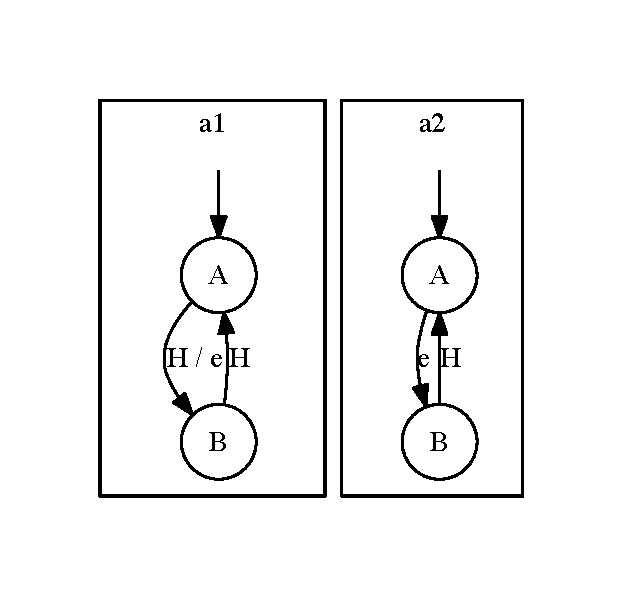
\includegraphics[width=0.5\textwidth]{figs/sync-ev1-model}\\
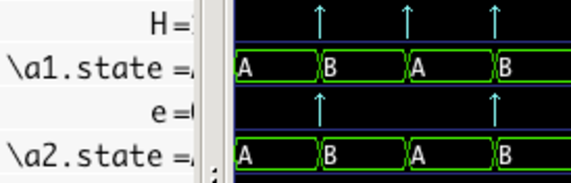
\includegraphics[width=0.7\textwidth]{figs/sync-ev1-chrono}
  \end{minipage}
\end{tabular}
  \caption{Illustration of instantaneous synchronisation}
  \label{fig:sync-ev1}
\end{figure}

\medskip
\textbf{Ephemeral synchronisation} means that if an event emitted by a FSM when taking a
transition is not awaited by another FSM it is simply ``lost''. In other words, events are never
memorised. This is illustrated in Fig.~\ref{fig:sync-ev2}.  In this example, the first occurence of
event \texttt{e} is lost because FSM \texttt{a2} is not waiting for it when it is emitted by FSM
\texttt{a1} at the first occurrence of event \texttt{H}.  As a result, the transition of \texttt{a2}
from state \texttt{B} to state \texttt{C} only occurs at second occurrence of \emph{e}, when
\texttt{a2} is in state \texttt{B}.

\begin{figure}[h]
  \centering
\begin{tabular}[c]{cc}
  \begin{minipage}[b]{0.3\linewidth}
  \begin{lstlisting}[language=Rfsm]
fsm model A1(
  in h: event,
  out e: event)
{
  states: A, B, C;
  trans:
  | A -> B on h with e
  | B -> C on h
  | C -> A on h;
  itrans:
  | -> A ;
}

fsm model A2(
  in h: event,
  in e: event)
{
  states: A, B, C;
  trans:
  | A -> B on h
  | B -> C on e
  | C -> A on h;
  itrans:
  | -> A ;
}
  \end{lstlisting}
  \end{minipage} &
  \begin{minipage}[b]{0.7\linewidth}
\begin{lstlisting}[language=Rfsm]
input H : event = sporadic(10, 20, 30, 40, 50)
shared e : event

fsm a1 = A1(H,e)
fsm a2 = A2(H,e)
\end{lstlisting}
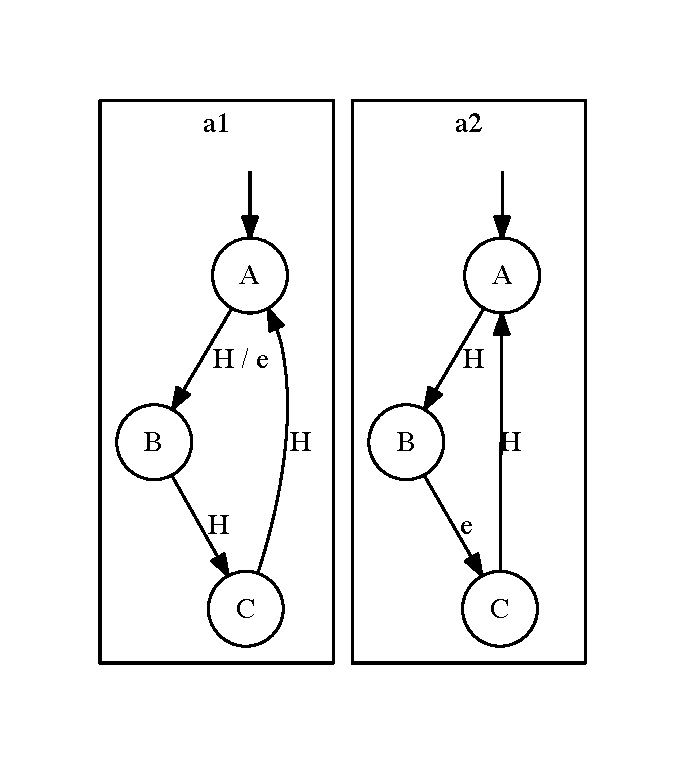
\includegraphics[width=0.5\textwidth]{figs/sync-ev2-model}\\
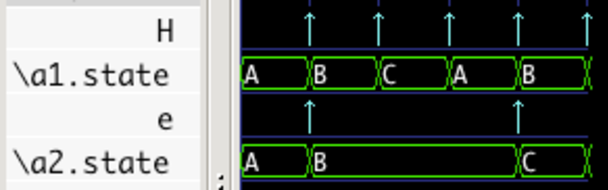
\includegraphics[width=0.7\textwidth]{figs/sync-ev2-chrono}
  \end{minipage}
\end{tabular}
  \caption{Illustration of ephemeral synchronisation}
  \label{fig:sync-ev2}
\end{figure}

\medskip \textbf{Note}. The semantics of event synchronisation described here is somehow related
to that of \emph{rendez-vous} supported by certain programming languages. But it is definitely not
equivalent. The latter enforces that \emph{both} transitions, the emitting and the
receiving one, are taken together. This means in particular that if there's no transition waiting
for the emitted event, the emitting transition will \emph{not} be taken (in other words, the source
FSM will block). This is not the case here. In this situation, and as explained above, the emitted
event will be simply ignored (``lost''). Emitting an event can never prevent a transition to be
taken in our semantics.

\medskip \textbf{Implementation issues}.  The semantics of events presented here is that implemented
by the \texttt{rfsmc} simulator. For various reasons, it may not fully supported all compiler
backends.  The support of shared events in the SystemC backend, for example, is fragile and has not
yet fully tested\footnote{It relies on the insertion of zero-time \texttt{wait} instructions.}. It
is completely lacking in the VHDL backend (VHDL implementation of FSMs can only be triggered by a
single, external, \texttt{clock} signal).  Finally, the \emph{event} mechanism provided by most
of real-time operating systems (as abstracted by \verb|notify_ev()| and \verb|wait_ev()|
pseudo-primitives used in the code generated by the C backend) may not obey the semantics provided
here (most of OS-supported events are \emph{memorized} when they are not awaited for when emitted in
particular). The concept of event provided by the RSFM language must therefore be viewed as a basic
and abstract \emph{modeling} tool, to be refined afterwards at the implementation level.

\subsubsection*{Synchronisation using shared variables}

The semantics associated to shared variables is that
of \emph{instantaneous broadcast}. This means that any modification of the value of a shared variable by a
FSM is immediately viewed by the other FSMs. More precisely, if a reaction of a FSM modifies the
value of a shared value, the new value can enable, \emph{in the same global reaction}, the
transition of another FSM. This is illustrated in Fig.~\ref{fig:sync-sv1}. Here, both \texttt{a1}
and \texttt{a2} react to event \texttt{H}. When \texttt{a1} and \texttt{a2} are in state \texttt{S1} this is possible
only because the modification of the shared variable \texttt{v} made by \texttt{a1} is immediately
visible and hence can enable the transition of \texttt{a2}.

\begin{figure}[h]
  \centering
\begin{tabular}[c]{cc}
  \begin{minipage}[b]{0.4\linewidth}
  \begin{lstlisting}[language=Rfsm]
fsm model A1(
  in h: event,
  out v: bool)
{
  states: S1, S2;
  trans:
  | S1 -> S2 on h with v:=1
  | S2 -> S1 on h with v:=0;
  itrans:
  | -> S1 with v:=0;
}
fsm model A2(
  in h: event,
  in v: bool)
{
  states: S1, S2;
  trans:
  | S1 -> S2 on h when v=1
  | S2 -> S1 on h; 
  itrans:
  | -> S1 ;
}
  \end{lstlisting}
  \end{minipage} &
  \begin{minipage}[b]{0.6\linewidth}
\begin{lstlisting}[language=Rfsm]
input H: event = sporadic(10,20,30,40)
shared V: bool

fsm a1 = A1(H,V)
fsm a2 = A2(H,V)
\end{lstlisting}
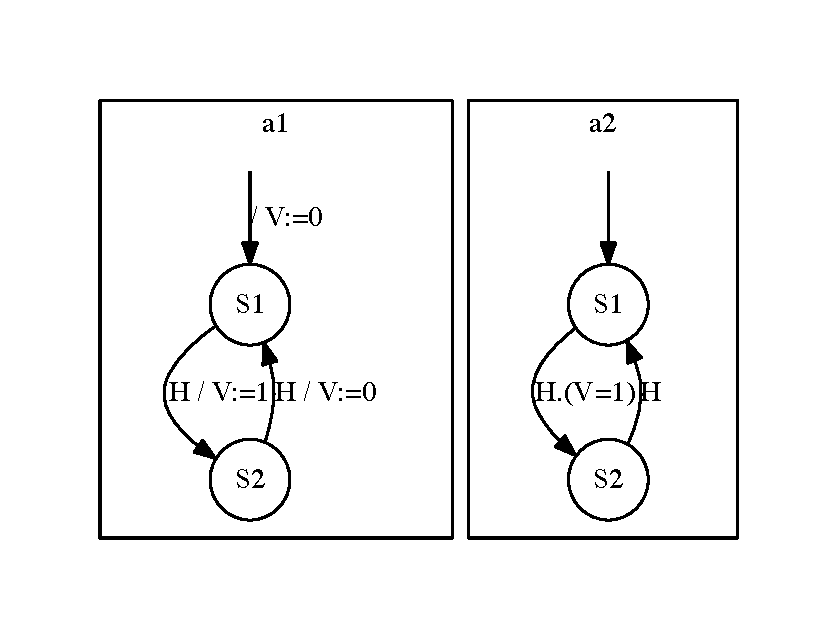
\includegraphics[width=0.7\textwidth]{figs/sync-sv1-model}
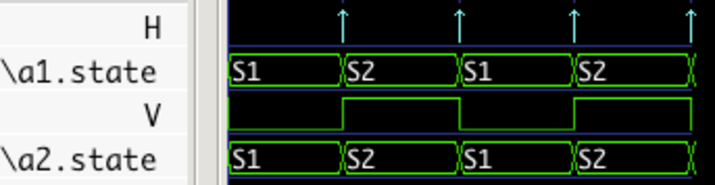
\includegraphics[width=0.7\textwidth]{figs/sync-sv1-chrono}
  \end{minipage}
\end{tabular}
  \caption{Illustration of instantaneous broadcast of shared variables}
  \label{fig:sync-sv1}
\end{figure}

\bigskip Because shared variables are, by definition, memorized, they can used to implement
\emph{defered synchronisation}, \emph{i.e.} the situation where a FSM emits an event which will be used
\emph{later} by another FSM (shared events cannot be used in this case since, as described above,
non-awaited events are not memorized and hence lost). This is illustrated in
Fig.~\ref{fig:sync-sv2}. Here, \texttt{a1} set variable \texttt{v} to 1 when going from state
\texttt{S1} to \texttt{S2} but \texttt{a2} only detects this when going from state \texttt{S2} to
\texttt{S3}, reseting the variable to 0 \emph{en passant}. In effect, \texttt{a1} has emitted a
event which has been memorized and caught latter by \texttt{a2}.

\begin{figure}[h]
  \centering
\begin{tabular}[c]{cc}
  \begin{minipage}[b]{0.4\linewidth}
  \begin{lstlisting}[language=Rfsm]
fsm model A1(
  in h: event,
  out v: bool)
{
  states: S1, S2, S3;
  trans:
  | S1 -> S2 on h with v:=1
  | S2 -> S3 on h
  | S3 -> S1 on h;
  itrans:
  | -> S1 with v:=0;
}

fsm model A2(
  in h: event,
  inout v: bool)
{
  states: S1, S2, S3;
  trans:
  | S1 -> S2 on h
  | S2 -> S3 on h when v=1
                  with v:=0
  | S3 -> S1 on h;
  itrans:
  | -> S1 ;
}
  \end{lstlisting}
  \end{minipage} &
  \begin{minipage}[b]{0.6\linewidth}
\begin{lstlisting}[language=Rfsm]
input H: event = sporadic(10,20,30)
shared v: bool

fsm a1 = A1(H,v)
fsm a2 = A2(H,v)
\end{lstlisting}
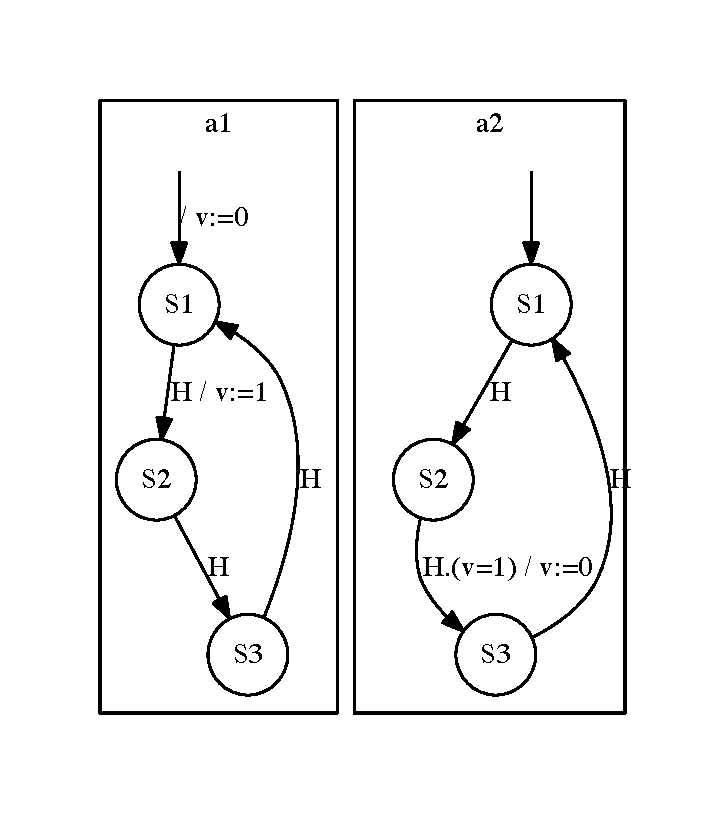
\includegraphics[width=0.7\textwidth]{figs/sync-sv2-model}
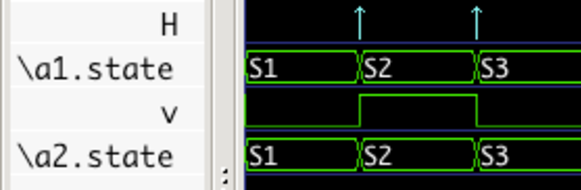
\includegraphics[width=0.7\textwidth]{figs/sync-sv2-chrono}
  \end{minipage}
\end{tabular}
  \caption{Using a shared variable to implement memorized events}
  \label{fig:sync-sv2}
\end{figure}

\medskip \textbf{Implementation issues}.  
The semantics of instantaneous broadcast for variables is the most intuitive one at the modelisation
level is the default one for simulation. However, and as for events, this semantics is not supported
by all compiler backends. 

For the SystemC backend, support of instantaneous broadcast is supported by means of
automatic insertion of zero-time delta-cycles and is therefore fragile.

It is \emph{not} supported by the VHDL backend because shared variables are (currently)
implemented as \emph{shared signals}, for which any modification at a given cycle is only visible
at the next clock cycle. 

Shared variables are implemented as global variables by the C backend. When the
corresponding code is used to define concurrent tasks for a real-time operating system, the
instantaneous broadcast hypothesis cannot in general be assumed (because the delay separating writes
and reads of such a variable depends of the scheduler and cannot be predicted).

% \medskip The \emph{instantaneous broadcast} interpretation can be replaced by a \emph{defered
%   broadcast} one by calling the compiler with the \verb|-no_inst_bcast| option. Any modification to
% a shared variable made by a FSM during a reaction will then not be visible by other FSMs at the same
% reaction but at the next one. This is illustrated for example in Fig.~\ref{fig:sync-vp1b} which
% shows the simulation results of the program listed in Fig.~\ref{fig:sync-vp1} when passing this
% option to the compiler. Here, the modification of the shared variable \texttt{v} operated by the
% transition from \texttt{s1} to \texttt{s2} of \texttt{a1} is \emph{not} viewed by \texttt{a2} at the
% same occurrence of the \texttt{H} event, but only at the next one.
 
% \begin{figure}[htbp]
%   \centering
% 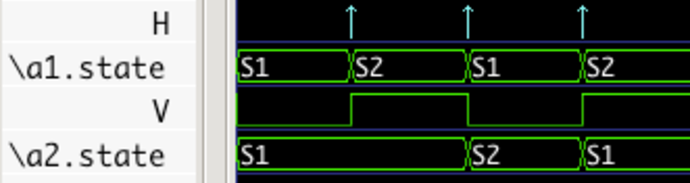
\includegraphics[width=0.6\textwidth]{figs/sync-vp1b}
%   \caption{Simulation results for the program of Fig.~\ref{fig:sync-vp1} when disabling the
%     instantaneous broadcast interpretation}
%   \label{fig:sync-vp1b}
% \end{figure}

% The \verb|-no_inst_bcast| option is supported both by the SystemC and VHDL backend. When using the
% latter, it makes the simulation result obtained by the VHDL simulator identical to those obtained by
% the simulator.

\section{FSM instances}
\label{sec:fsm-instances}

The description of the system is carried out by instanciating
%-- and, possibly, inter-connecting --
previously defined FSM models.

\medskip
Instanciating a model creates a copy of the corresponding FSM for which
\begin{itemize}
\item the parameters of the model are bound to their actual value,
\item the declared inputs and outputs are connected to global inputs, outputs or shared
  objects.
\end{itemize}

\medskip
The syntax for declaring a model instance is as follows~:

\begin{center}
\framebox{\lstinline[language=Rfsm]'fsm inst_name = model_name<param_values>(actual_ios)'} 
\end{center}

where
\begin{itemize}
\item \emph{inst\_name} is the name of the created instance,
\item \emph{model\_name} is the name of the instanciated model,
\item \emph{param\_values} is a comma-separated list of values to be assigned to the formal
  (generic) parameters,
\item \emph{actual\_ios} is a comma-separated list of global inputs, outputs or shared objects to be
  connected to the instanciated model.
\end{itemize}

Binding of parameter values and IOs is done by position. Of course the number and respective types
of the formal and actual parameters (resp. IOs) must match.

\medskip
For example, the last line of the program given in Listing~\ref{lst:rfsm-gensig}

\begin{center}
\example{\lstinline[language=Rfsm]'fsm g = gensig<3>(H,E,S)'}
\end{center}

creates an instance of model \verb|gensig| for which \verb|n=3| and whose inputs (resp. output) are
connected to the global inputs (resp. output) \texttt{H} and \texttt{E} (resp. \texttt{S}).

\medskip
In the current version, paramater values are limited to scalar values (\texttt{int}s,
\texttt{bool}s, \texttt{char}s and \texttt{float}s). 

% For example, provided that globals \verb|Top|, \verb|Clic|, \verb|SimpleClic| and \verb|DoubleClic|
% have been previously declared with the correct type,  writing

% \begin{lstlisting}[language=Rfsm,frame=single,basicstyle=\small]
% fsm c1 = ctlr<5>(Top,Clic,SimpleClic,DoubleClic)
% \end{lstlisting}

% will create an instance of the FSM model described in
% Fig.~\pageref{fig:fsm-model-ex} named \verb|c1| and for which \verb|D=5|.

\section{Constants}
\label{sec:constants}

Global constants can be defined using the following syntax~:  

\begin{center}
\framebox{\lstinline[language=Rfsm]|constant name : <type> = <value>|}
\end{center}

\noindent
where
\begin{itemize}
\item \emph{type} is the type of the defined constant (currently limited to
  \verb|int|, \verb|bool|, \verb|char|, \verb|float| and arrays of such types,
\item \emph{value} is the value of the constant.
\end{itemize}

Global constants have a global scope and hence can be used in any FSM model or instance.

\section{Functions}
\label{sec:functions}

Conditions and actions associated to FSM transitions can use globally defined functions. An example
is given in listing~\ref{lst:rfsm-heron}\footnote{This example can be found in directory
  \texttt{examples/std/single/heron} in the distribution.}. The FSM described here computes an approximation
of the square root of its input \verb|u| using Heron's classical algorithm. Successive approximations are computed in
state \verb|Iter| and the end of computation is detected when the square of the current
approximation \verb|x| differs from the argument (\verb|a|) from less than a given threshold
\verb|eps|. For this, the model uses the global function \verb|f_abs| defined at the beginning of
the program. This function computes the absolute value of its argument and is used twice in the
definition of the FSM model \verb|heron|, for defining the condition associated to the two
transitions going out of state \verb|Iter|.

\begin{lstlisting}[language=Rfsm,frame=single,numbers=left,caption=An RFSM program using a global
  function definition,label={lst:rfsm-heron},float]
function f_abs(x: float) : float { return x < 0.0 ? -.x : x }

fsm model heron<eps: float>(
  in h: event,
  in start: bool,
  in u: float,
  out rdy: bool,
  out niter: int,
  out r: float)
{
  states: Idle where rdy=1, Iter where rdy=0;
  vars: a: float, x: float, n: int;
  trans:
  | Idle -> Iter on h when start=1 with a:=u, x:=u, n:=0
  | Iter -> Iter on h when f_abs((x*.x)-.a)>=eps with x:=(x+.a/.x)/.2., n:=n+1
  | Iter -> Idle on h when f_abs((x*.x)-.a)<eps with r:=x, niter:=n;
  itrans:
  | -> Idle;
}

input H : event = periodic (10,10,200)
input U : float = value_changes (5:2.0)
input Start : bool = value_changes (0:0, 25:1, 35:0)
output Rdy1, Rdy2 : bool
output R1, R2 : float
output Niter : int

fsm h = heron<0.00000001> (H,Start,U,Rdy2,Niter,R2)
\end{lstlisting}

\medskip
\step The general form for a function definition is 

\begin{center}
\framebox{\lstinline[language=Rfsm]| function name (<arg\_1>:<type\_1>, ..., <arg\_n>:<type\_n>)\ :\ <type\_r> \{ return <expr> \}|}
\end{center}

\noindent
where
\begin{itemize}
\item \lstinline[language=Rfsm]|<arg_i>| (resp. \lstinline[language=Rfsm]|<type_i>|) is the name
  (resp. type) of the i$^{th}$ argument,
\item \lstinline[language=Rfsm]|<type_r>| is the type of value returned by the function,
\item \lstinline[language=Rfsm]|<expr>| is the expression defining the function value.
\end{itemize}

\medskip
\step Functions can only return one result and cannot use local variables. There are therefore more
like \emph{macros} in the C language and are typically used to improve readability of the programs.

\section{Types and type declarations}
\label{sec:types}

Types present in RFSM programs belong to two categories~: builtin types and user defined types.

\medskip
\textbf{Builtin types} are : \texttt{bool}, \texttt{int}, \texttt{float}, \texttt{char}, \texttt{event} and
\texttt{array}s.

\medskip
\step Objects of type \texttt{bool} can have only two values : \texttt{0} (false) and \texttt{1} (true).

\step Values of type \texttt{char} are
denoted using single quotes. For example, for a variable \verb|c| having type \verb|char|~:
\begin{center}
  \example{\lstinline[language=Rfsm]|c := 'A'|}
\end{center}
They can be converted from/to they internal representation as integers using the "\verb|::|" \emph{cast}
operator. For example, if \verb|c| has type \verb|char| and \verb|n| type \verb|int|, then 
\begin{center}
  \example{\lstinline[language=Rfsm]|n := 'A'::int; c:=(n+1)::char|}
\end{center}
assigns value 65 to \verb|n| (ASCII code) and, then, value \verb|'B'| to \verb|c|.

% \begin{table}[h]
% %\begin{minipage}[c]{1.0\linewidth}
% \small
% \begin{center}
% \begin{tabular}{|l|l|} \hline
% {\tt int}       & {\tt + - * / mod = != > < >= <=} \\  \hline
% {\tt bool}      & {\tt = !=} \\ \hline 
% {\tt enumeration}     & {\tt = !=} \\  \hline
% \end{tabular}
% \caption{Operations on types}
% \label{tab:type-ops}
% \end{center}
% %\end{minipage}
% \end{table}

\medskip
\step The type \texttt{int} can be refined using a \emph{size} or a \emph{range annotation}. The
type \verb|int<sz>|, where \verb|sz| is an integer, is the type of integers which can be encoded using
\verb|n| bits. The type \verb|int<min:max>|, where both \verb|min| and \verb|max| are integers, is
the type of integers whose value ranges from \verb|min| to \verb|max|. The size and range limits,
can be given as litteral constants (ex: \verb|8|) or as parameter values\footnote{Provided, of
  course, that the corresponding parameter as type \texttt{int}.}, as for the type of the
variable \texttt{k} in Listing~\ref{lst:rfsm-gensig}.

\medskip
\step Supported operations on values of type \texttt{int} are described in Table~\ref{tab:int-ops}.
If \verb|n| is an integer and \verb|hi| (resp. \verb|lo|) an integer expression then \verb|n[hi:lo]|
designates the value represented by the bits \verb|hi|...\verb|lo| in the binary representation of
\verb|n|. Bit ranges can be both read (ex: \verb|x=y[6:2]|) or written (ex: \verb|x[8:4]:=0|). The
syntax \verb|n[i]|, where \verb|n| is an integer is equivalent to \verb|n[i:i]|. The \emph{cast}
operator (\verb|::|) can be used to combine integers with different sizes (for example, if \verb|n|
has type \verb|int<16>| and \verb|m| has type \verb|int<8>|, writing \verb|n:=n+m| is not allowed
and must be written, instead, \verb|n:=n+m::int<16>|. Note that the
logical ``or'' operator is denoted ``\verb+||+'' because the single ``\verb+|+'' is already used in
the syntax.

\begin{table}[h]
\begin{center}
\begin{tabular}{|l|l|} \hline
\verb|+|, \verb|-|, \verb|*|, \verb|/|, \verb|%| (modulo) & arithmetic operations \\ \hline 
\verb|>>|, \verb|<<| & (logical) shift right and left \\ \hline 
\verb|&|, \verb+||+, \verb|^| & bitwise and, or and xor \\ \hline 
\verb|[.:.]| & bit range extraction (ex: \verb|n:=m[5:3]|) \\ \hline 
\verb|[.]| & single bit extraction (ex: \verb|b:=m[4]|) \\ \hline 
\verb|::| & resize (ex: \verb|n::int<8>|) \\ \hline 
\end{tabular}
\caption{\label{tab:int-ops}Builtin operations on integers}
\end{center}
\end{table}

\medskip
\step The operations on values of type \texttt{float} are : "\verb|+.|", "\verb|-.|", "\verb|*.|" and
"\verb|/.|" (the dot suffix is required to distinguish them from the corresponding operations on
\texttt{int}s).

\medskip
\step Arrays are 1D, fixed-size collections of \verb|int|s, \verb|bool|s, \verb|char|s or \verb|float|s. Indices
range from 0 to \verb|n-1| where \verb|n| is the size of the array. For example,
 \verb|int array[4]| is the type describing arrays of four integers. If \verb|t| is an object
  with an array type, its cell with index $i$ is denoted \verb|t[i]|.

\bigskip
\textbf{User defined types} are either \emph{type abbreviations}, \emph{enumerations} or
\emph{records}.

\medskip
\step Type abbreviations are introduced with the following declaration
\begin{center}
  \framebox{\lstinline[language=Rfsm]{type typename = type_expression}}
\end{center}
Each occurrence of the defined type in the program is actually substituted by the corresponding type
expression.
% Type expressions in type abbreviations are currently limited to builtin types.

\medskip
\step Enumerated types  are introduced with the following declaration
\begin{center}
  \framebox{\lstinline[language=Rfsm]|type typename = enum \{ C1, ..., Cn \}|}
\end{center}
where \verb|C1|, \ldots, \verb|Cn| are the enumerated values, each being denoted by an identifier
starting with an uppercase letter. For example : 
\begin{center}
  \example{\lstinline[language=Rfsm]|type color = \{ Red, Green, Orange \}|}
\end{center}

\medskip
\step Record types are introduced with the following declaration
\begin{center}
  \framebox{\lstinline[language=Rfsm]|type typename = record \{ fid1: ty1, ..., fidn: tyn \}|}
\end{center}
where \verb|fid1|, \ldots, \verb|fidn| and \verb|ty1|, \ldots, \verb|tyn| are respectively the name
and type of each record field For example : 
\begin{center}
  \example{\lstinline[language=Rfsm]|type coord = record \{ x: int, y: int\}|}
\end{center}

Individual fields of a value with a record type can be accessed using the classical ``dot''
notation. For example, with a variable \verb|c| having type \verb|record| as defined above :
\begin{center}
  \example{\lstinline[language=Rfsm]|c.x := c.x+1|}
\end{center}

% \medskip The listing in Fig.~\ref{fig:fsm-model-ex} gives an example of a FSM model declaration. The
% declared model is that of a simplified mouse controler. It has two inputs, \verb|Top| and
% \verb|Clic|, and two outputs, \verb|SimpleClic| and \verb|DoubleClic|. All inputs an and outputs are
% of type \verb|event|. Input \verb|Top| is here supposed to be periodic and hence provide an time
% base. Whenever an event occurs on the input \verb|Clic|, an event is emitted either on
% \verb|DoubleClic| or \verb|SimpleClic| depending on whether the \verb|Clic| event is followed by
% another before \verb|D| events occur on the \verb|Top| input, where \verb|D| is a parameter of the
% model. The description of the behavior employs two states, named \verb|Idle| and \verb|Wait|, an
% internal variable, \verb|ctr|, and four transitions rules, listed in the \verb|trans:| section.  The
% first rules says that a transition from state \verb|Idle| to state \verb|Wait| happens whenever and
% event occurs on input \verb|Clic| and that the internal variable \verb|ctr| is then reset to 0. The
% second rule says that a transition from state \verb|Wait| to state \verb|Idle| happens whenever and
% event occurs on input \verb|Clic| and that an event is then emitted on output \verb|DoubleClic|. The
% third rule says that a transition from state \verb|Wait| to itself happens whenever and event occurs
% on input \verb|Top| provided that, at this instant, the value of variable \verb|ctr| is less than
% \verb|D-1|. The variable \verb|ctr| is then incremented. The fourth and last rule says that a
% transition from state \verb|Wait| to state \verb|Idle| happens, emitting an event on output
% \verb|SimpleClic|, whenever and event occurs on input \verb|Top| and that, at this instant, the
% value of variable \verb|ctr| is equal to \verb|D-1|. Finally, the initial transition, given after
% the keyword \verb|itrans:| designates the state \verb|Idle| as the initial state (with no associated
% action here). 

% A graphical representation of this FSM is given on the right in Fig.~\ref{fig:fsm-model-ex} (this
% diagram has been automatically generated by the RFSM compiler, as explained in
% Chap.~\ref{chap:using}). 

% \begin{figure}[t]
%   \begin{minipage}[b]{0.6\linewidth}
%    \centering
% \begin{lstlisting}[language=Rfsm,frame=single,basicstyle=\small]
% fsm model ctlr<D:int> (
%   in Top: event,
%   in Clic: event,
%   out SimpleClic: event,
%   out DoubleClic: event)
%   {
%   states:  Idle, Wait;
%   vars:  ctr: int<0..D>;
%   trans:
%     Idle -- Clic | ctr:=0 -> Wait,
%     Wait -- Clic | DoubleClic -> Idle,
%     Wait -- Top.ctr<D-1 | ctr:=ctr+1 -> Wait,
%     Wait -- Top.ctr=D-1 | SimpleClic -> Idle;
%   itrans: -> Idle;
%   }
% \end{lstlisting}
%   \end{minipage}
%   \begin{minipage}[b]{0.4\linewidth}
%    \includegraphics[height=5cm]{figs/mousectlr-dot}
%    \centering
%   \end{minipage}
% \hfill
%   \caption{Example of an FSM model description (with its graphical representation)}
%   \label{fig:fsm-model-ex}
% \end{figure}

%%% Local Variables: 
%%% mode: latex
%%% TeX-master: "rfsm_um"
%%% End: 
